\documentclass[compress,red]{beamer}
\usetheme{Warsaw}
\useoutertheme[subsection=false]{smoothbars}

\usepackage{helvet}
\usepackage{graphicx}
\usepackage{booktabs}
\usepackage{hyperref}
\usepackage{url}

\usepackage{remreset}% tiny package containing just the \@removefromreset command
\makeatletter
\@removefromreset{subsection}{section}
\makeatother
\setcounter{subsection}{1}

\title[FOSS at CERN: Drivers in the Kernel]%
	{Free and Open Source Software at CERN:\\
	Integration of Drivers in The Linux Kernel}
\author[David Cobas et al.]{%
	Juan David Gonz\'alez Cobas, Samuel Iglesias Gons\'alvez,\\
	Julian Howard Lewis, Javier Serrano, Manohar Vanga\\
		(CERN, Geneva),\\
	Emilio G. Cota (Columbia University, NY; formerly at CERN),\\
	Alessandro Rubini, Federico Vaga (University of Pavia)}
\date{ICALEPCS'2011}

\begin{document}

\begin{frame}
\titlepage
\end{frame}

\section{The tsi148 bridge}
\begin{frame}{CERN Controls System Front End Computers (FECs)}

The controls system relies on FECs on several form factors/buses,
most of them based on Single-Board Computers (SBCs)

\begin{itemize}
\item Number of FECs: 1140
\item Number of VME crates: 710
\end{itemize}

For the VME crates, the ongoing renovation process gives
\begin{itemize}
\item CES RIO2/RIO3 SBCs with PowerPC CPUs runing
LynxOS (around 605 crates by August 2011), to
\item MEN-A20 SBCs with Intel CPUs running real-time
Linux (around 105 by August 2011).
\end{itemize}
\end{frame}


\begin{frame}{MEN A20 and the TSI148 chip and driver}

The MEN A20 SBC is an Intel Core 2 Duo-based board interfacing to the
VME bus via a Tundra TSI148 PCI-X to VME bridge chip.

% wget http://www.men.de/docs-ext/products/images/img_photo/01a020-_hi.jpg
% ftp://ftp.ruby-lang.org/pub/ruby/1.8/ruby-1.8.7-p352.tar.gz
\begin{center}
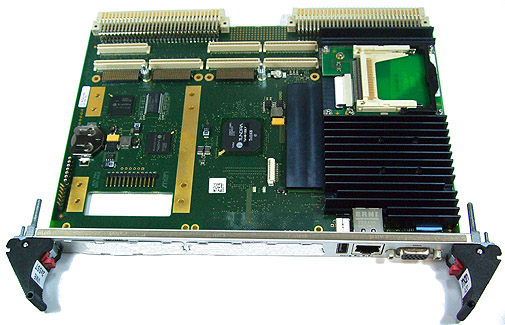
\includegraphics[height=4cm]{01a020-_hi.pdf} \qquad
\includegraphics[height=2.75cm]{p_tundra_Tsi148-HR.pdf}
\end{center}
\end{frame}

\begin{frame}{A driver for the \texttt{tsi148}}

Some data about our driver for the \texttt{tsi148} PCI-X to VME bridge.
\begin{itemize}
\pause\item Developed at CERN in spring 2009 (S\'ebastien Dugu\'e)
\pause\item Maintained and extended by Emilio G. Cota during 2010
\pause\item Currently maintained by Manohar Vanga (see below)
\pause\item API via exported symbols (kernel) and old-style \texttt{ioctl()} (user) interface.
\pause\item Backward compatible at the API level with the original LynxOS CES
    library (well, almost) and offering a newer API as well
\end{itemize}

\pause Beginning as an \textcolor{red}{in-house}
and \textcolor{red}{CERN-centric} development
\end{frame}

\begin{frame}{Why going upstream? (2010)}

By mid-2010, the decision is taken to submit the driver for acceptance
in the Linux kernel main tree. Motivation:

\begin{itemize}
\item Smoother maintenance in the (frequent) case of\\
	kernel API changes\\
  (see \texttt{Documentation/stable\_api\_nonsense.txt} in the kernel
  tree).
\item Widespread distribution of the code base, which can then be
    enhanced and get contributed by researchers
\item Contributing back in return to the many benefits the FOSS community
    gives us.
\end{itemize}
The original motivations were \textcolor{red}{more ideological than
practical}
\end{frame}

\begin{frame}{How the driver was merged (2010--2011)}

\pause
\begin{block}{Who, when, how}
\begin{itemize}
\item Merge process with pre-existing \texttt{./staging/}
driver for the Tundra Universe and TSI148 chips
\item Four-round process (Emilio G. Cota, Manohar Vanga)
\item Core device model modifications accepted by mid 2011
\end{itemize}
\end{block}

\pause
\begin{block}{Lessons learned}
\begin{itemize}
\item It is hard, LKML and maintainers are tough
\item One must be prepared to compromise (design, APIs, tools)
\item One must build a reputation slowly
\item Requires \textcolor{red}{patience}
\end{itemize}
\end{block}
\end{frame}

\begin{frame}{Lessons learned}
But the most important one was that our initial motivations
\pause
\begin{center}
\textcolor{red}{turned out to be wrong}
\end{center}
\pause
\begin{center}
\Huge Why?
\end{center}
\end{frame}

\section{FMC boards}

\begin{frame}{A typical data acquisition application: carrier}
\begin{center}
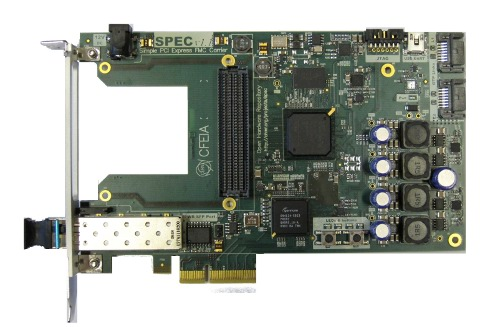
\includegraphics[height=0.8\textheight]{spec.pdf}
\end{center}
\end{frame}

\begin{frame}{A typical data acquisition application: mezzanine}
\begin{center}
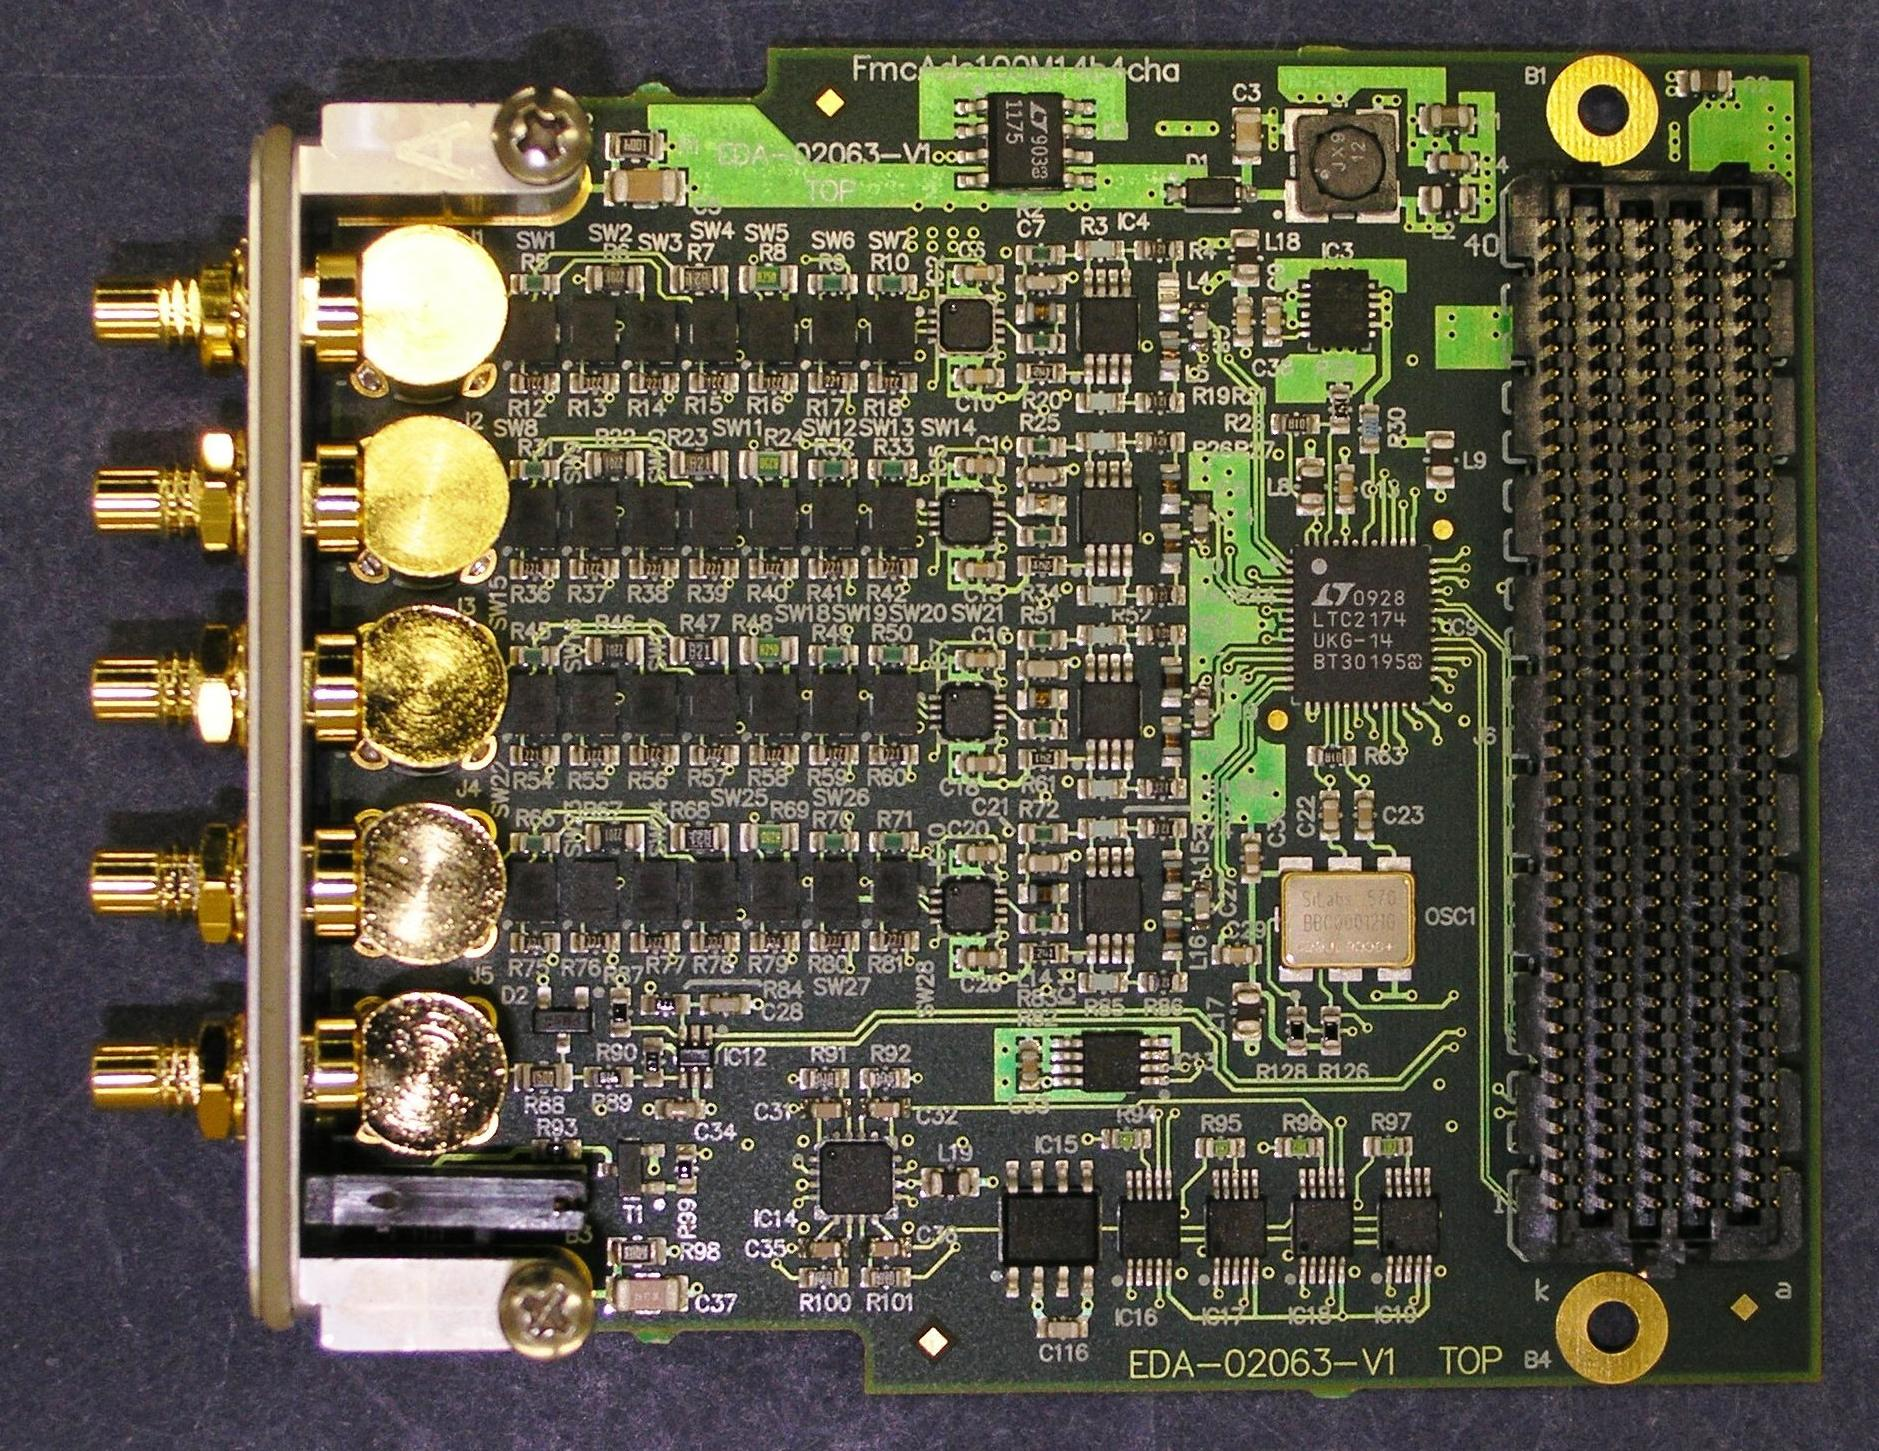
\includegraphics[rotate=180,height=0.7\textheight]{fmcadc.pdf}
\end{center}
\end{frame}

\begin{frame}{The FMC family of boards}

This is a substantial part of our standard HW kit, currently under
development\\
(see \url{http://www.ohwr.org/projects/fmc-projects}).

\begin{itemize}
\item carriers in PCIe and VME format
\item simple mezzanines with electronics for ADCs, DACs, DIO and endless
    other applications
\item circuitry in the mezzanine
\item FPGA application logic in the carrier
\item \emph{logic in the FPGA is organized as a set of IP cores
    interconnected through an internal bus named
    \textcolor{red}{Wishbone}}
\end{itemize}
\end{frame}

\begin{frame}{Architecture of the FMC drivers}
\includegraphics[height=0.8\textheight]{THCHMUST04f1.pdf}
\end{frame}

\begin{frame}{Drivers for the FMC family}
The main concepts for the design of these drivers are
\begin{itemize}
\pause
\item modular structure that reflects the core structure of the firmware
\pause
\item one-to-one mapping driver $\leftrightarrow$ core (usually)
\pause
\item ability to dynamically load bitstreams by application
\end{itemize}

\pause
On the whole, the driver for the carrier board acts as a basic firmware
loader and a bridge driver (with device enumeration
\emph{\`a la PCI)} between the host bus (PCIe, VME) and the FPGA
interconnection bus

\pause
It will be (we hope) the first Wishbone bus driver in the mainstream
kernel $\Rightarrow$ will to go upstream, timeliness
\end{frame}

\section{The \texttt{zio} framework}

\begin{frame}{BE/CO data acquisition modules}
   \begin{tiny}
   \begin{tabular}{llllll}
       \toprule
	\textbf{Module}& \textbf{Type}& \textbf{Channels}&
	\textbf{Resolution}& \textbf{Max. Speed}& \textbf{Bus} \\
       \midrule
	VMOD-12E8/16    &  Analog input  & 8/16ch & 12b    & 15us/sample & VME/PCI  \\
	VD80            &  Analog input  & 16ch   & 16b    & 200kS/s     & VME  \\
	SIS3300         &  Analog input  & 8ch    & 12/14b & 100MS/s     & VME  \\
	SIS3302         &  Analog input  & 8ch    & 16b    & 100MS/s     & VME  \\
	SIS3320         &  Analog input  & 8ch    & 12b    & 250MS/s     & VME  \\
	``Fast'' FMC ADC&  Analog input  & 4ch    & 14b    & 100Ms/s	 & VME/PCIe (WB)  \\
	``Slow'' FMC ADC&  Analog input  & 8ch    & 16b    & 100kS/s     & VME/PCIe (WB)  \\
       \midrule
	CVORB V4        &  Analog output & 16ch   &  16b   &  5us/sample & VME 	 \\
	VMOD-12A2/4     &  Analog output & 2ch    &  12b   &  10us/sample& VME/PCI \\
	CVORG           &  Analog output & 2ch    &  14b   &  100 MS/s   & VME  \\
       \midrule
	VMOD-TTL        &  Digital I/O   & 20ch   & 1b     & n/a         & VME/PCI \\
	CVORA           &  Digital I/O   & 32ch   & 1--32b & 100Mhz	 & VME \\
       \bottomrule
   \end{tabular}
   \end{tiny}
\end{frame}

\begin{frame}{Industrial I/O frameworks}

\pause
\begin{block}{In Linux staging area}
\begin{itemize}
\item Comedi
\item IIO
\end{itemize}
\end{block}

\pause
\begin{block}{Drawbacks}
\begin{itemize}
\item do not suit our needs
\item interfaces are cumbersome
\end{itemize}
\end{block}

\pause
\begin{block}{Then \texttt{zio} comes}
\begin{itemize}
\item Alessandro Rubini and Federico Vara, main developers
\item Integration mainstream \emph{ab initio}
\item See (soon) under \url{http://www.ohwr.org/}
\pause\item \textcolor{red}{Clean design conforming to Linux kernel practice}
\end{itemize}
\end{block}

\end{frame}

\begin{frame}{Next candidates for (\texttt{zio}) integration}

CERN-developed drivers for
\begin{itemize}
\pause
\item Struck SIS33xx ADCs
\pause
\item Tews TPCI200/TVME200 carries plus IPOCTAL serial boards
\pause
\item all the CERN BE/CO-supported FMC boards in the Open Hardware Repository
\pause
\item timing receivers, White Rabbit, etc.
\end{itemize}
\end{frame}

\section{Conclusions and The Ultimate Goal}

\begin{frame}{Why did we do it?}

It gave us much more than we thought in the first place
\begin{itemize}
\pause
\item Smoother maintenance in the (frequent) case of\\
	kernel API changes.
\item Widespread distribution of the code base.
\item Contributing back to the the FOSS community.
\pause \color{red}
\item Very strict process of peer review of the code by knowledgeable
    and specialised maintainers.
\pause
\item Input (consulting!) from the topmost experts in the field.
\pause
\item Avoidance of suboptimal, \emph{ad hoc} solutions in favour of the
    best ones from the technical point of view.
\pause
\item Use of best practice and bleeding-edge tools selected by
    experienced programmers, \emph{e.g.} \texttt{git}, \texttt{sparse}
    and \texttt{coccinelle}.
\end{itemize}
\end{frame}

\end{document}
